\chapter{INTRODUCTION}
\label{ch:intro}

NEW~\cite{particle_data_group_review_2020}.

% \textbf{Motivation---why you should read this thesis
% What is this thesis about?}
% At first glance, the Universe appears to be an overwhelmingly vast and complicated place.
% However upon closer inspection, it is comprised of only a few different kinds of fundamental particles.
% Particle physics has given rise to the Standard Model (SM) which mathematically describes these constituents and their interactions with each other.
The Universe, while overwhelmingly vast, is comprised of a curiously small number of indivisible particles.
As shown in Fig.~\ref{fig:particular_table}, these \emph{elementary} particles can be split into two main kinds: a mere 12 \emph{matter} particles (green and pink) that comprise all detectable matter and 4 \emph{force} particles (red) that convey forces between the matter particles.
Although it is fascinating to wonder how can so much diversity can arise from just 16 ``simple'' building blocks, it is the mission of particle physicists to understand the underlying mathematical structure that describes Nature in as simple---and accurate---a theory as possible.
The best theory developed so far is called the Standard Model (SM) of particle physics (see Chapter~\ref{ch:theory} for a mathematical overview).
% Universe metastability.
%%%%%%%%%%%%%%%%%%%%
\begin{figure}[hbtp]
    \centering
    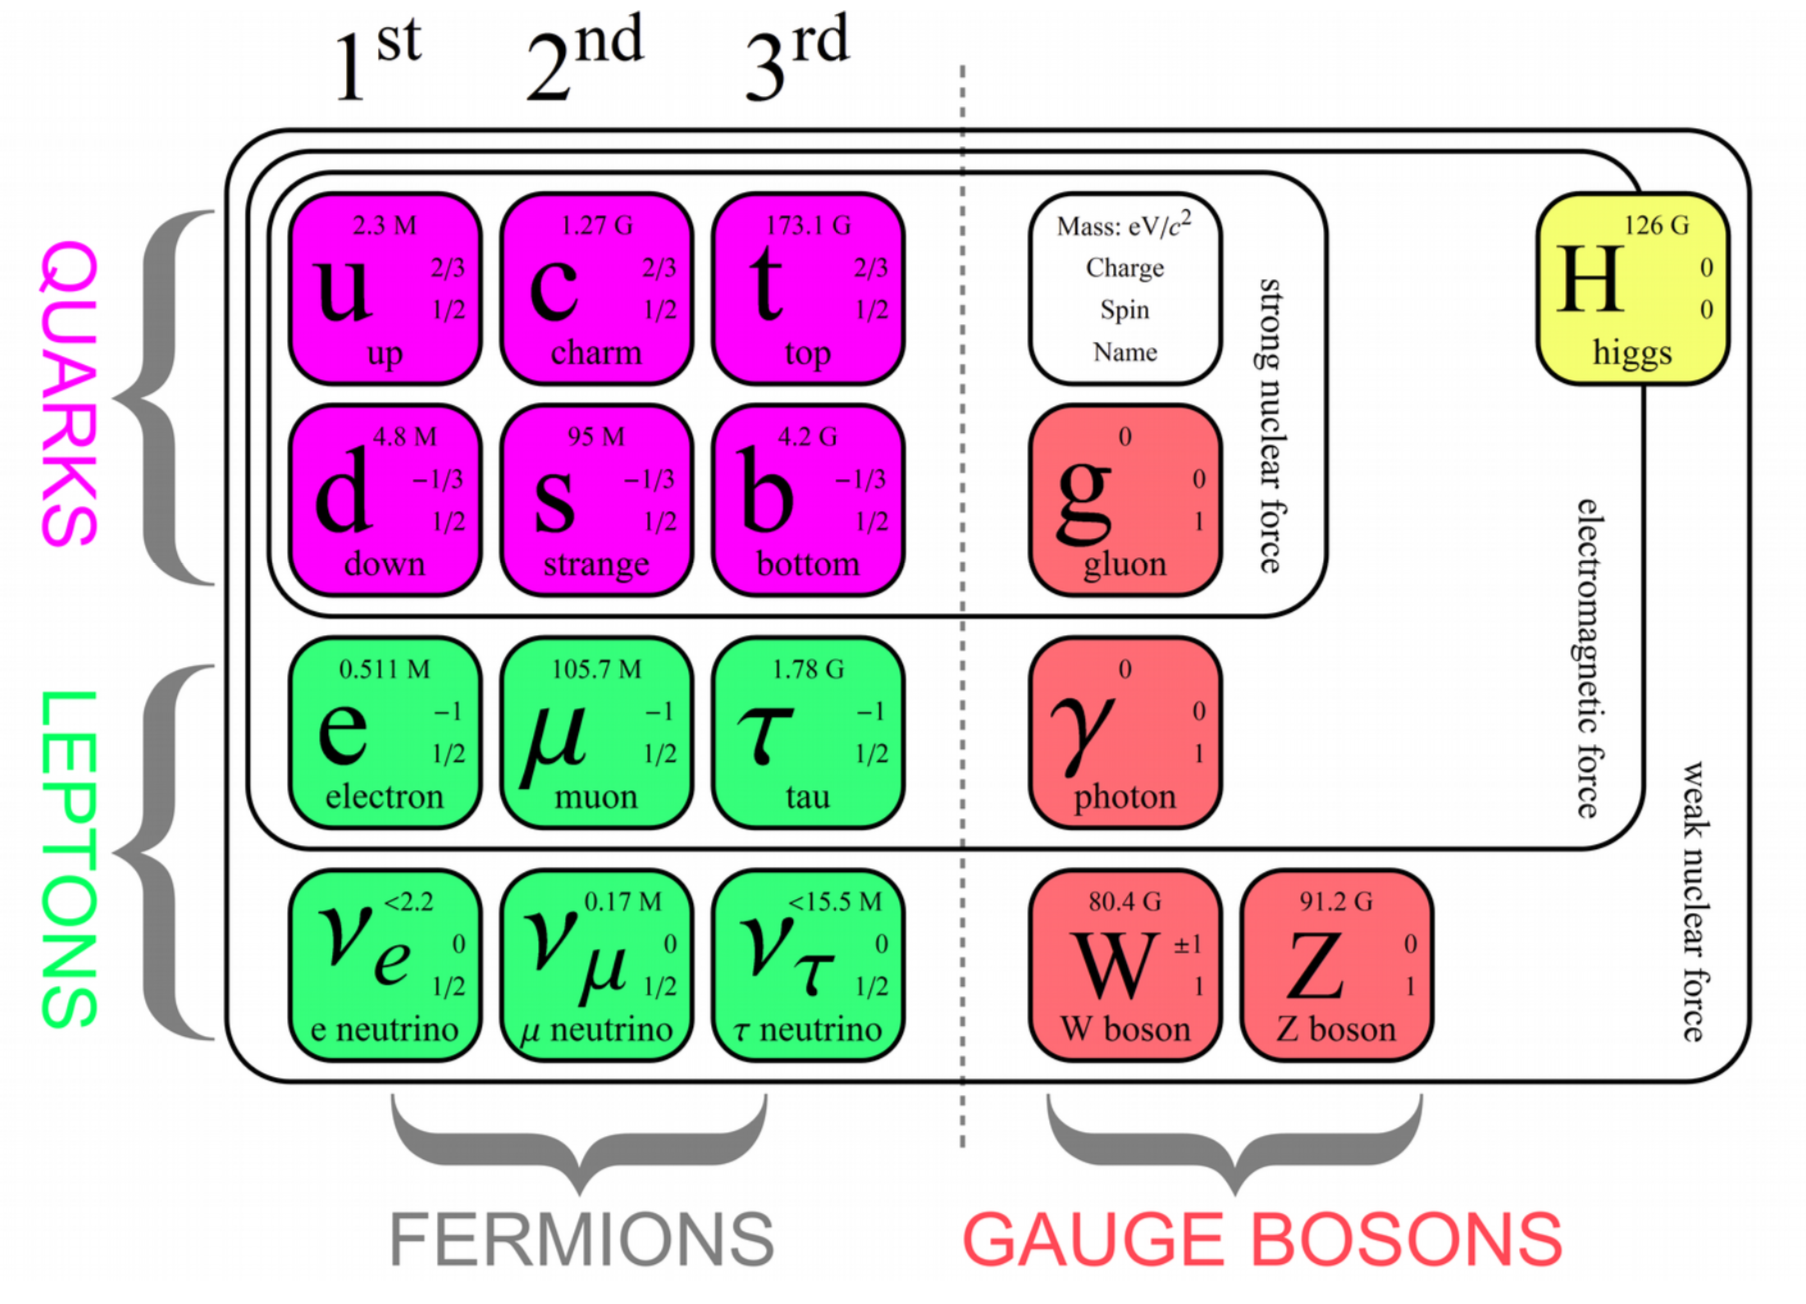
\includegraphics[width=15cm,height=10cm,keepaspectratio]{figures/sm/particular_table_updated.png}
        \caption{
        TODO
        }
        \label{fig:particular_table}
\end{figure}
%%%%%%%%%%%%%%%%%%%%
% , the SM accurately describes most of the properties of the eleme

% Although the SM will be mathematically outlined in Chapter~\ref{ch:theory}, it is 
The SM has bore witness to many triumphs over its approximately 70-year development:
it predicted the existence of quarks which were experimentally confirmed in the mid-1970s;
it predicted the existence of the tau neutrino which was experimentally confirmed in 2000;
its most groundbreaking prediction was experimentally confirmed on July 4, 2012---almost exactly 10 years ago from the date of this dissertation writing---when the ATLAS and CMS collaborations announced the discovery of the Higgs boson~\cite{Chatrchyan:2012xdj}.

% Many properties of these particles---and their interactions with each other---are accurately described by the standard model (SM) of particle physics.
% Problematically though, the SM predicts that the gauge bosons (the particles which convey forces) particles are massless.
% The most significant triumph of the SM occurred on July 4$^\text{th}$ TODO:comma? 2012 when the ATLAS and CMS collaborations announced the discovery of the ``missing puzzle piece'' of the SM---the Higgs boson.
% This discovery confirmed the SM's prediction that there should exist, which date back to 1964 via the Brout-Englert-Higgs mechanism

% In the SM, particle interactions are conveyed by way of 3 fundamental forces, the strong, weak, and electromagnetic forces, while the 4th force---gravity---is neglected due to its negligible contribution at nuclear distances.
% The seed of the most successful triumph of the SM dates back to 1964, when physicists Robert Brout, François Englert, and Peter Higgs , which occurred on July 4th, 2012, was possible its most spectacular: the when the Higgs boson was  The prediction capabilities of the SM are 
% strong, weak, and electromagnetic interactions
% By understanding the rules by which these particles interact, we can ;
% this is the aim of the Standard Model (SM) of Particle Physics. 
% The Standard Model (SM) is an impressively accurate mathematical theory which describes the fundamental particles of the universe and the rules for their possible interactions.
% 
%  are described mathematically by the impressively accurate Standard Model (SM) of Particle Physics.
% Although there are four fundamental forces of nature, the SM takes into account three of the four forces in nature:
The Higgs boson (\PH) is a critical piece of the SM because, without it,  it is the quantum excitation of the so-called Higgs field, an all-pervasive field throughout spacetime 
Before 

It is necessary to scrutinize the properties of this new particle to check whether it truly is the \PH predicted by the SM---or perhaps something else entirely.
Thus, the Large Hadron Collider accelerates protons to near-light speeds 

A major shortcoming of the SM is its inability to predict the masses of these particles.

The SM was not able to predict the masses of these particles until 1964 when the Brout-Englert-Higgs mechanism suggested that 
It wasn't until 1964 that the Brout-Englert-Higgs mechanism gave a self-consistent way to :
by breaking the electroweak gauge symmetry of the vacuum would give rise to non-zero masses of the weak gauge bosons.
This would yield a secondary effect too:
there should exist a fundamental scalar boson which is the quantum of the so-called ``Higgs field''.
On July 4th, 2012, this Higgs boson was discovered.

This dissertation presents the world's most precise measurement of the Higgs boson mass (\mH) to date, using proton-proton collision data from the LHC Run 2, collected and analyzed by the CMS Experiment.
The value of \mh has been measured previously TODO:CITE LOTS OF PEEPS~\cite{Chatrchyan:2013lba} but it is important to always strive for lower uncertainties (\ie to increase the precision) on the mass value, since the very stability of our universe theoretically depends on \mH, as shown in Fig.~\ref{fig:universe_stability}.
% Additionally, the value of \mh is one of the free parameters of the SM and is theoretically linked to the very stability of our universe.
Furthermore, the value of \mh sets limits on the masses of most of the other elementary particles.
% Universe metastability.
%%%%%%%%%%%%%%%%%%%%
\begin{figure}[hbtp]
    \centering
    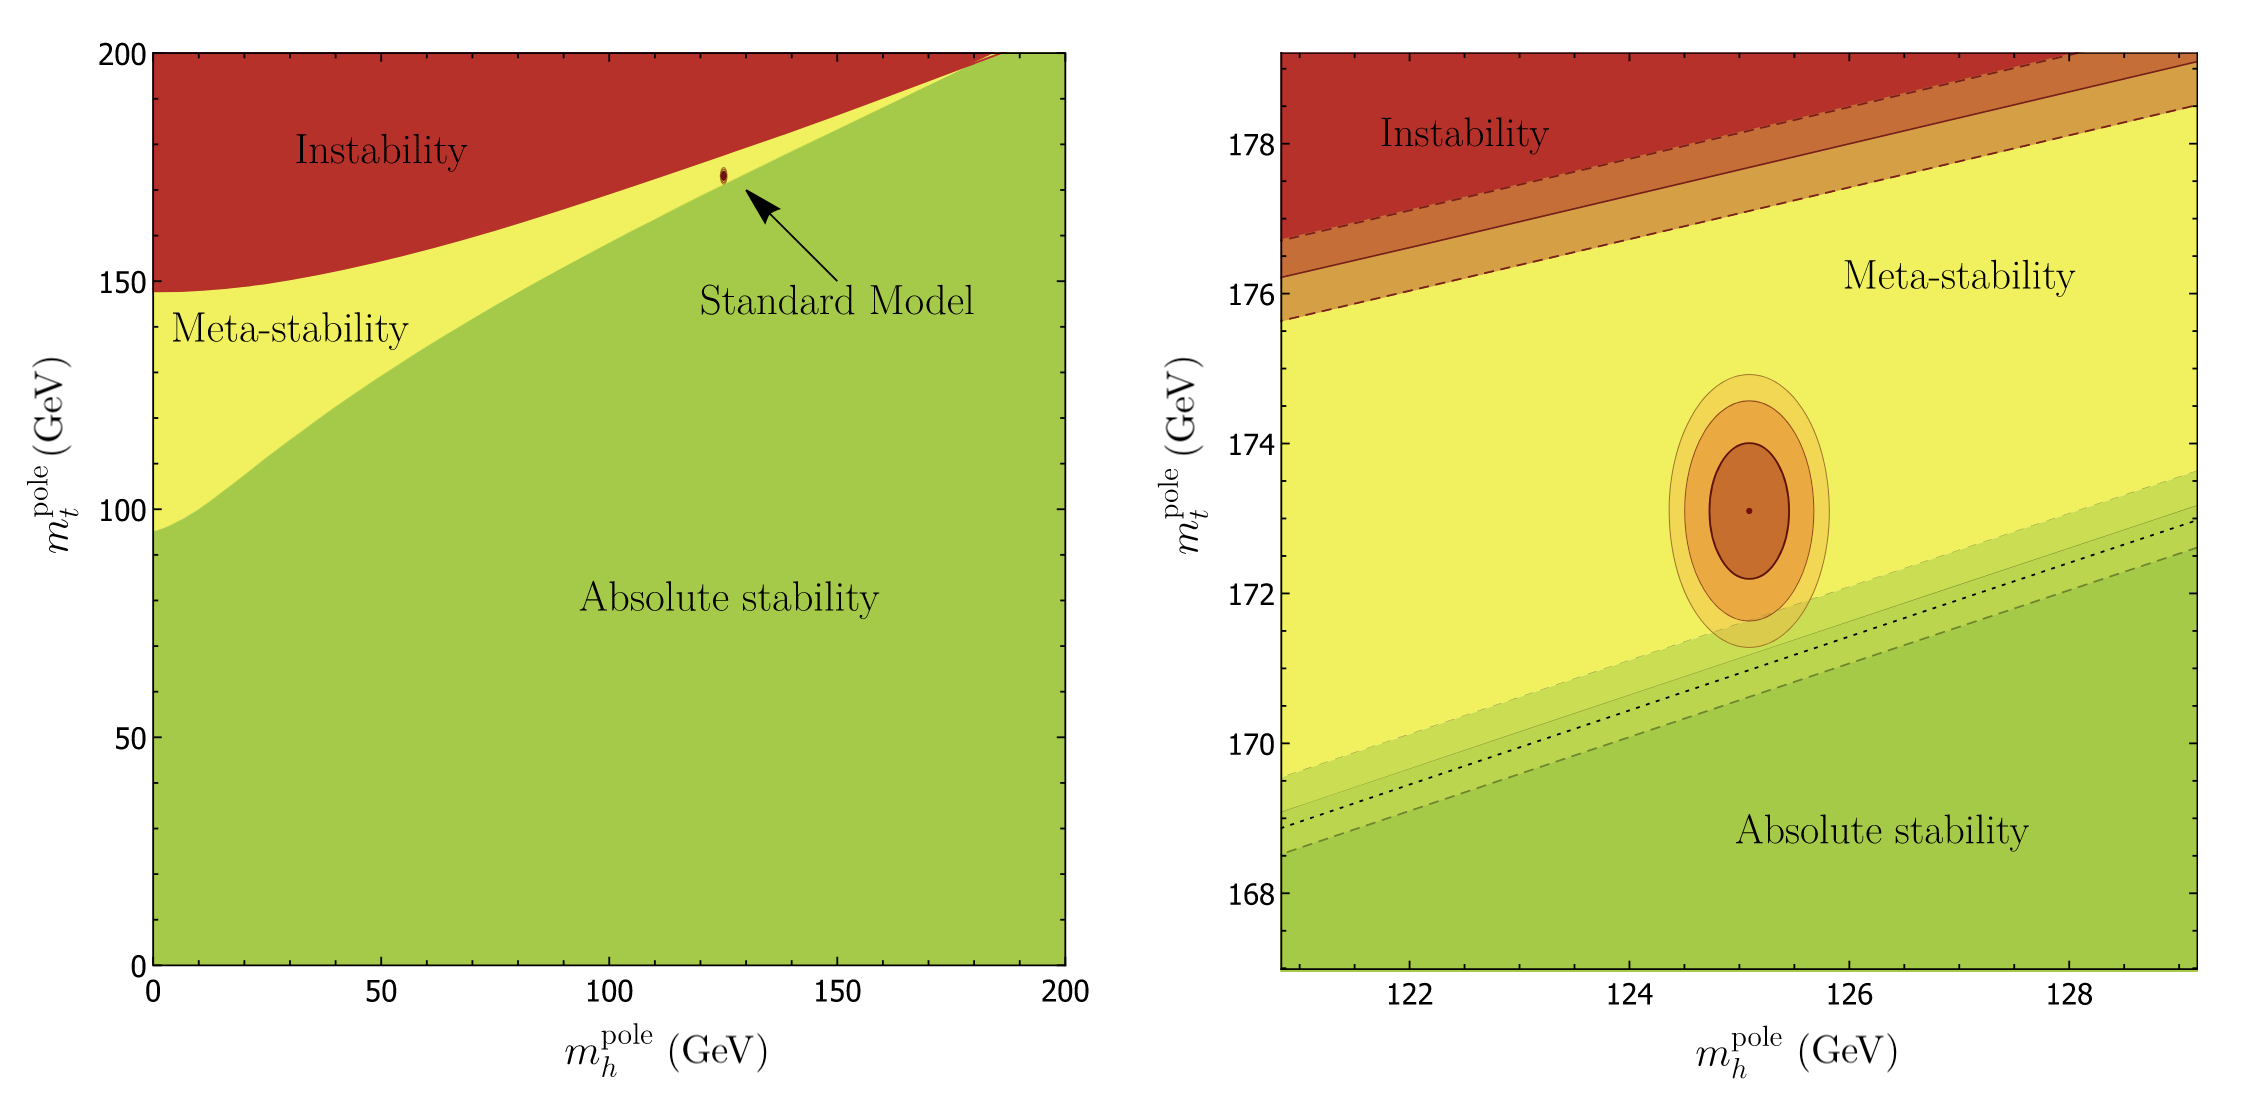
\includegraphics[width=15cm,height=10cm,keepaspectratio]{figures/intro/mtop_vs_mH_universestability.png}
        \caption
        [Theoretical stability regions of our universe.]
        {
            (Left) Theoretical stability regions of our universe based on the pole masses of the top quark $\left( \mass{t}^\text{pole} \right)$ and Higgs boson $\left( \mass{h}^\text{pole} \right)$.
            (Right) A closeup of the SM region of the left plot.
            The contours represent the 68\%, 95\%, and 99\% confidence levels based on the experimental uncertainties of $\mass{t}^\text{pole}$ and $\mass{h}^\text{pole}$.
            Plots taken from~\cite{univ_stab} and units added to all axes.
        }
        \label{fig:universe_stability}
\end{figure}
%%%%%%%%%%%%%%%%%%%%

The measurement of \mH presented in this dissertation utilizes the following improvements compared to previous measurements:
\begin{itemize}
    % More data.
    \item Utilizing nearly four times as much collected data from Run 2 $\left( \lumiint = \lumiruntwo \right)$ \vs the data used for the 2016 measurement $\left( \lumiint = \lumisixteen \right)$.
    % Four final states (instead of three).
    \item Four final-state categories are used: \fourmu, \foure, \twoetwomu, \twomutwoe.
    In previous measurements, the last two final states (the mixed-flavor states) were combined, when truly they have different kinematical properties (depending on into which lepton pair the \Zone decayed):
    different peak widths (instrumental resolutions), different signal efficiencies, and different relative levels of reducible background.
    % Using UL reco (better electron pT resolution).
    \item Ultra-Legacy (UL) reconstruction is used for muon, electron, photon, and jet tracks.
    This signficantly improves electron momenta and improves the other particle momenta, though to a lesser degree.
    % Vertex constraint.
    \item The measurements of muon \pt are improved by constraining the muon tracks to originate from the interaction vertex (also called a \emph{vertex constraint}).
    \item When extracting the value of \mH in past measurements, a 3D $\text{pdf} \left( \mfourl, \mfourlerr, \Dkinbkg \right)$ was built into a factorized form
    $f \left( \mfourl, \mfourlerr \middlepipe \mH \right)   \cdot   g\left( \Dkinbkg \middlepipe \mfourl \right)$,
    which was later found to contain an existing correlation between \mfourlerr and \Dkinbkg.
    To account for this correlation, now the events are split into 9 categories based on the per-event \emph{relative} mass uncertainty $\left( \relmfourlerr \right)$ and, for each, a 2D $\text{pdf} \left( \mfourl, \Dkinbkg \middlepipe \mh \right)$ is built.
    % Z1 mass constraint.
    % \item Just as was done in the 2016 \mH measurement~\cite{}TODO:CITE, a \Zone mass constraint is imposed on events with the \fourmu and \twomutwoe final states to improve the momenta of the two muons comprising the \Zone.
    % The improvement here is that now the muon tracks are constrained to come from the interaction vertex in the fit (sometimes called a \emph{vertex constraint}).
    \item The systematic uncertainties on electron and muon momentum scales $\left( \pt^{\Pe, \mu} \right)$ are reduced, thanks to a more detailed analysis on the uncertainties.
    This has the additional effect of significantly reducing the uncertainty on the per-event four-lepton mass resolution.
\end{itemize}

This dissertation is organized into the following chapters:
Chapter~\ref{ch:intro} (\emph{this chapter}) discusses the importance and motivation for measuring the mass of the Higgs boson;
Chapter~\ref{ch:theory} introduces the standard model (SM) of particle physics and its mathematical framework, including the Brout-Englert-Higgs (BEH) mechanism;
Chapter~\ref{ch:lhc};
Chapter~\ref{ch:cms};
Chapter~\ref{ch:higgs_mass};
Chapter~\ref{ch:dilep_res};
Finally, Chapter~\ref{ch:conclusion}.
